\documentclass[11pt,twoside,a4paper]{article}
\usepackage[T1]{fontenc}
\usepackage[utf8]{inputenc}
\usepackage[top=20mm, bottom= 15mm, left=15mm, right=15mm]{geometry}
\usepackage{amsmath}
\usepackage{dsfont}
\usepackage{calc}
\usepackage{comment}
\usepackage{pythontex}
\usepackage{tikz}
\usetikzlibrary{automata,positioning}
\newcommand{\mylabel}[1]{#1\hfill}
\renewenvironment{itemize}
  {\begin{list}{$\triangleright$}{%
   \setlength{\parskip}{0mm}
   \setlength{\topsep}{.4\baselineskip}
   \setlength{\rightmargin}{0mm}
   \setlength{\listparindent}{0mm}
   \setlength{\itemindent}{0mm}
   \setlength{\labelwidth}{2ex}
   \setlength{\itemsep}{.4\baselineskip}
   \setlength{\parsep}{0mm}
   \setlength{\partopsep}{0mm}
   \setlength{\labelsep}{1ex}
   \setlength{\leftmargin}{\labelwidth+\labelsep}
   \let\makelabel\mylabel}}{%
   \end{list}\vspace*{-1.3mm}}
\parindent0ex
\parskip1.5ex
\newcounter{quesito}
\newenvironment{question}{\addtocounter{quesito}{1}\par\textbf{Quesito \thequesito.\kern1ex}}{\vspace{0.5\parskip}}
\newenvironment{xquestion}{\bigskip\addtocounter{quesito}{1}\bigskip\bigskip\par\textbf{Quesito \thequesito.\kern1ex}}{\vspace{\parskip}}
\newenvironment{answer}{\par\textbf{Risposta\quad}}{\vspace{\parskip}}

\pagestyle{empty}
\excludecomment{xquestion}
\excludecomment{answer}

\begin{document}
\colorbox{blue!10}{\begin{minipage}{\textwidth}
Matematica e BioStatistica con Applicazioni Informatiche\\
Esercitazione in aula del 10 gennaio 2018
\end{minipage}}



\begin{pycode}
import random
random.seed('daxtxsdsxssme')
ESAME = False
\end{pycode}

    
\begin{question}
\def\Pr{{\rm Pr\,}}
\def\pyl#1{\py{latex(#1) } }
\everymath{\displaystyle}
\def\nicefrac#1#2{#1/#2}
\renewcommand{\arraystretch}{1.3}
\begin{pycode}
from sympy import *
random.seed(9409934)
while True :
    tp  =  random.sample( [1,2,3,4,5,6], 6 ) 
    pab, pac, pba, pbc, pca, pcb = [Integer(i) for i in tp] 
    if pab+pac<=10 and pba+pbc<=10 and pca+pcb<=10: break
    
M = Matrix([  [10-pab-pac, pba,        pca       ],
              [pab,         10-pba-pbc, pcb      ],
              [pac,         pbc,        10-pca-pcb] ] )
    
a, b, c = symbols('a b c')

M1 = Rational(1,10)*M - eye(3)
M1 = M1.row_insert(3, Matrix([ [1, 1, 1] ] ) )
M1 = M1.col_insert(3, Matrix([0, 0, 0, 1] ) )
equilibrio = solve_linear_system(M1, a, b, c)

\end{pycode}
Un rospo vive in uno stagno e passa le sue giornate saltando tra tre foglie di ninfea 
che indichiamo con {\sf a}, {\sf b}, e {\sf c}. Ogni ora salta da foglia una all'altra 
con probabilità riassunte nel diagramma sottostante (la probabilità di restare nello 
stesso punto è lasciata implicita). 

\hfil
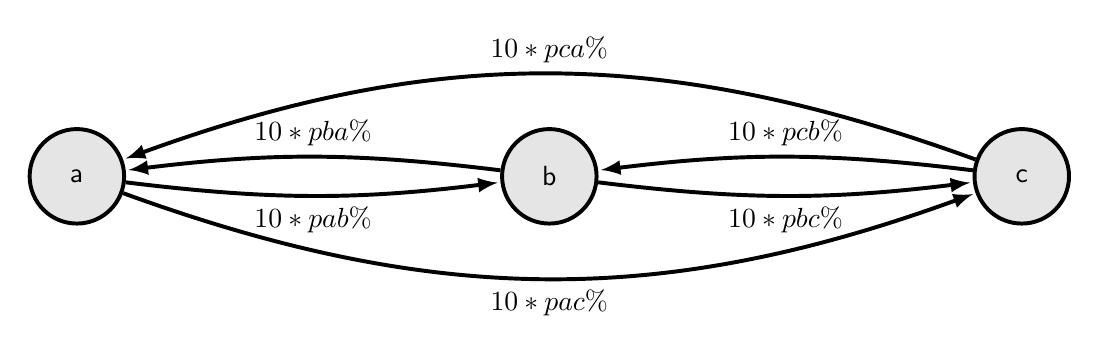
\begin{tikzpicture}[font=\sffamily]
  
  % Setup the style for the states
  \tikzset{node style/.style={state, 
                              minimum width=1.2cm,
                              line width=0.5mm,
                              fill=gray!20!white}}

  % Draw the states
  \node[node style] at (0, 0)     (a)     {a};
  \node[node style] at (6, 0)     (b)     {b};
  \node[node style] at (12, 0)    (c)     {c};

  % Connect the states with arrows
  \draw[every loop,
        auto=right,
        line width=0.5mm,
        >=latex]
      (a) edge[bend right=20, auto=right]  node {$\py{10*pac}\%$} (c)
      (a) edge[bend right=7, auto=right]   node {$\py{10*pab}\%$} (b)
      (b) edge[bend right=7, auto=right]   node {$\py{10*pba}\%$} (a)
      (b) edge[bend right=7, auto=right]   node {$\py{10*pbc}\%$} (c)
      (c) edge[bend right= 7, auto=right]  node {$\py{10*pcb}\%$} (b)
      (c) edge[bend right=20, auto=right]  node {$\py{10*pca}\%$} (a);
\end{tikzpicture}

Osservando il rospo in un momento qualsiasi, lo troveremo in {\sf a}, {\sf b}, o {\sf c} con probabilità 
rispettivamente $\py{equilibrio[a]}$, $\py{equilibrio[b]}$, e $\py{equilibrio[c]}$. 
Supponiamo che il rospo sia in {\sf a} al tempo $t=1$ 

\begin{itemize}
\item[1.] Qual è la probabilità che al tempo $t=2$ il rospo passi a {\sf b}~?

\item[2.] Qual è la probabilità che al tempo $t=0$ il rospo fosse in {\sf c}~?

\item[3.] Qual è la probabilità che al tempo $t=3$ il rospo si trovi in {\sf c}~?

\end{itemize}

Esprimere il risultato come rapporto di numeri interi.

\begin{answer}

Siano $R_t$ le variabili aleatorie che danno la posizione del rospo al tempo $t$.

Dal testo inferiamo che $\Pr(R_t={\sf a})=\py{equilibrio[a]}$, $\Pr(R_t={\sf b})=\py{equilibrio[b]}$, e $\Pr(R_t={\sf c})=\py{equilibrio[c]}$

Dal diagramma inferiamo 

$\Pr(R_{2}={\sf b}~|~R_1={\sf a})\ =\kern1.2ex${\color{blue}$\py{pab/10}$\hfill Risposta 1}

$\Pr(R_{1}={\sf a}~|~R_0={\sf c})\ =\kern1.2ex\py{pca/10}$

Quindi

$\Pr(R_0={\sf c}~|~R_1={\sf a})
\ =\ \frac{\Pr(R_1={\sf a}\,|\,R_0={\sf c})\cdot\Pr(R_0={\sf c})}{\Pr(R_1={\sf a})}
\ =\ \frac{(\py{pca/10})\cdot(\py{equilibrio[c]})}{\py{equilibrio[a]}}$

$\phantom{\Pr(R_0={\sf c}~|~R_1={\sf a})}
\ =\kern1.2ex${\color{blue}$\py{pca*equilibrio[c]/(equilibrio[a]*10)}$\hfill Risposta 2}


Ci sono tre casi mutualmente escusivi per il percorso del rospo ai tempo $1,2,3$ 
che elenchiamo con le rispettive probabilità.

{\sf a,\ b,\ c}\hfill$\pyl{pab/10}\cdot\pyl{pbc/10} = \pyl{(pab * pbc) / 100}$

{\sf a,\ a,\ c}\hfill$\pyl{(10-pac-pab)/10}\cdot\pyl{pac/10} = \pyl{((10-pac-pab) * pac)/100}$

{\sf a,\ c,\ c}\hfill$\pyl{pac/10}\cdot\pyl{(10-pca-pcb)/10} = \pyl{(pac * (10-pca-pcb))/100}$


$\pyl{(pab * pbc) / 100} + \pyl{((10-pac-pab) * pac)/100} +  \pyl{(pac * (10-pca-pcb))/100} 
\ =\ $
{\color{blue}$\pyl{ (pab * pbc) / 100 + ((10-pac-pab) * pac)/100 +  (pac * (10-pca-pcb))/100}$\hfill Risposta 3}

\end{answer}
\end{question}
    

  
\begin{question}
\begin{pycode}
from scipy.stats import binom
n = random.choice([26,27,28,29])
k = random.choice([12,13,14,15])
t = random.choice(["t","u"])
risposta = round( 1- binom.cdf(k-1,n, 1/4), 4)
\end{pycode}
Consideriamo sequenze di $\py{n}$ caratteri dell'alfabeto $\{a,g,c,\py{t}\}$. 
Assumiamo che tutti i caratteri occorrano con la stessa probabilità indipendentemente dalla posizione.
Fissata una sequenza $s_0$, qual è la probabilità che un'altra sequenza $s_1$ 
scelta in modo indipendente coincida con $s_0$ in $\ge\py{k}$ posizioni?   

Esprimere il risutato numerico tramite (solo) le funzioni elencate in calce.
\begin{answer}
    
  $X\sim B(\py{n}, 1/4)$
  
  $\Pr(X\ge \py{k})\ =\ 1-\Pr(X\le \py{k-1})$
  \quad =\ 
  {\tt{\color{blue}  1 -  binom.cdf( $\py{k-1}$, $\py{n}$, 1/4 )}
  \ =\ 
  \py{risposta}}{\color{blue}\hfill Risposta}
\end{answer}
  \end{question}



\begin{question} % 33333333333333
\begin{pycode}
# dis = random.choice( [ '>', '<'])
dis =  '>'
if ESAME: dis = '<'

if dis == '<':
   dis_eq  = '\\le'
   adis    = '>'
   adis_eq = '\\ge'
   sign = '+'

if dis == '>':
   dis_eq  = '\\ge'
   adis    = '<'
   adis_eq = '\\le'
   sign = '-'

\end{pycode}
Vogliamo testare $H_0:\mu=\mu_0$ contro $H_A:\mu\py{dis}\mu_0$ per una popolazione distribuita normalmente con deviazione standard nota $\sigma$. Fissiamo una significatività $\alpha$ e una potenza $1-\beta$. L'effect-size che ci interessa è $\delta$.  Esprimere, in funzione dei parametri che assumiamo noti, le condizioni cui deve soddisfare il rango $n$ del campione.

\begin{answer}

{\color{blue}Il rango necessario è il minimo $n$ tale che $\displaystyle\Pr\bigg(Z\py{adis}\frac{x_\alpha-\mu_0\py{sign}\delta}{\sigma/\sqrt{n}}\bigg)\le\beta$

dove $x_\alpha$ tale che $\displaystyle\Pr\bigg(Z\py{dis_eq} \frac{x_\alpha-\mu_0}{\sigma/\sqrt{n}}\bigg)=\alpha$\hfill Risposta}


\end{answer}
\end{question}

{\color{red}\bfseries Il seguente quesito NON è stato assegnato in classe. Lo includo perché agli studenti che chiedevano suggerimento per la soluzione dell Quesito~3 ho erroneamente suggerito la soluzione di questo.}
   
\begin{question}
\begin{pycode}
from scipy.stats import nbinom
# n = random.choice([26,27,28,29])
# k = random.choice([12,13,14,15])
# t = random.choice(["t","u"])
risposta = round( 1- nbinom.cdf(k-1,n, 1/4), 4)
\end{pycode}
Consideriamo sequenze di caratteri dell'alfabeto $\{a,g,c,\py{t}\}$. 
Assumiamo che tutti i caratteri occorrano con la stessa probabilità indipendentemente dalla posizione.
Leggiamo due sequenze $s_0$ ed $s_1$ da sinistra a destra, qual è la probabilità che la prima differenza occorra non prima di $\py{k}$ caratteri (ovvero occorre al carattere  $\py{k}$ o ai seguenti)?   

Esprimere il risutato numerico tramite (solo) le funzioni elencate in calce.
\begin{answer}
    
  $X\sim NB(\py{n}, 1/4)$
  
  $\Pr(X\ge \py{k})\ =\ 1-\Pr(X\le \py{k-1})$
  \quad =\ 
  {\tt{\color{blue}  1 -  nbinom.cdf( $\py{k-1}$, $\py{n}$, 1/4 )}
  \ =\ 
  \py{risposta}}{\color{blue}\hfill Risposta}
\end{answer}
  \end{question}



\vfill\hrulefill\par
\begin{tabular}{@{}lll}
Formulario:& se $X\sim B({\tt n},{\tt p})$ & allora $E(X)=np$\\
           & se $X\sim NB({\tt n},{\tt p})$& allora $E(X)=n(1-p)/p$\\
\end{tabular}
\\[1ex]
Si assuma noto il valore delle seguenti funzioni della libreria {\tt scipy.stats\/} di  {\tt Python\/}\\
{\tt binom.pmf(k, n, p)} = $\Pr\big(X={\tt k}\big)$ dove $X\sim B({\tt n},{\tt p})$\\
{\tt binom.cdf(k, n, p)} = $\Pr\big(X\le{\tt k}\big)$ dove  $X\sim B({\tt n},{\tt p})$ \\
{\tt bimom.ppf(q, n, p)} = ${\tt k}$ dove ${\tt k}$ è tale che 
                           $\Pr\big(X\le{\tt k}\big)\cong{\tt q}$ per $X\sim B({\tt n},{\tt p})$\\
{\tt nbinom.xxx(\ldots)}, è l'analogo per $X\sim NB({\tt n},{\tt p})$.\\
{\tt norm.xxx(\ldots)}, è l'analogo per $Z\sim N(0,1)$.\\
\hfill{\tt t.xxx(\ldots, $\nu$)}, è l'analogo per $T\sim t(\nu)$.
\end{document}


